% This is manuscript_springer_lnns.tex
% Prepared for Springer LNNS (Lecture Notes in Networks and Systems) / LNCS format
% Compatible with llncs.cls

\documentclass[runningheads]{llncs}

\usepackage{graphicx}
\usepackage{amsmath,amssymb}
\usepackage{booktabs}
\usepackage{tabularx}
\usepackage{hyperref}
\usepackage{microtype}

\begin{document}

\title{Explainable Machine Learning for Chronic Kidney Disease Classification Using NHANES 2021--2023 Data: Feature Attribution Stability and Missing-Data Sensitivity}

\titlerunning{Explainable ML for CKD Classification: Attribution Stability}

\author{First Author\inst{1}\orcidID{0000-0000-0000-0000} \and
Second Author\inst{1}\orcidID{0000-0000-0000-0000} \and
Corresponding Author\inst{2,*}\orcidID{0000-0000-0000-0000}}

\authorrunning{F. Author et al.}

\institute{Department of Computer Science and Engineering, Institute / University, City, Country \and
Department of Biomedical Informatics and Computational Health, Institute / University, City, Country\\
\email{*corresponding.author@university.edu}}

\maketitle

\begin{abstract}
Chronic kidney disease (CKD) affects an estimated 10\% to 15\% of adults globally, yet early stages typically remain asymptomatic and unmanaged. Supervised learning models trained on routine clinical examinations offer potential for opportunistic risk screening. However, existing tabular benchmarks frequently suffer from target leakage by supplying direct diagnostic markers---such as serum creatinine or urinary albumin---as input features. Furthermore, post-hoc explanations generated by Shapley Additive Explanations (SHAP) are rarely audited for stability across data resamples or resilience under missing inputs. In this study, we evaluate non-leaking clinical and demographic variables from the Continuous National Health and Nutrition Examination Survey (NHANES) 2021--2023. We identify and resolve an artifact in the public dataset where 5,607 records lacking laboratory measurements (primarily pediatric participants aged $<12$ years) were misclassified as CKD-positive by default logic, yielding a verified cohort of 6,326 participants (3,592 non-CKD [56.8\%] and 2,734 CKD [43.2\%]). Quarantining seven target-defining features, we train Logistic Regression, Random Forest, and XGBoost across repeated stratified 5-fold cross-validation (25 folds) using 21 non-leaking predictors. TreeSHAP and LinearSHAP attributions are computed on out-of-fold validation splits, aggregated from one-hot levels back to parent variables, and assessed across all 300 pairwise fold combinations. Models are further stress-tested by injecting 10\% and 20\% synthetic Missing Completely at Random (MCAR) noise into validation sets. Across 25 folds, XGBoost achieved an ROC-AUC of $0.8456 \pm 0.0129$ and PR-AUC of $0.8246 \pm 0.0149$, closely tracked by L2-regularized Logistic Regression (ROC-AUC $0.8441 \pm 0.0123$) and Random Forest (ROC-AUC $0.8406 \pm 0.0123$). Global SHAP rankings identified chronological age, blood urea nitrogen, systolic blood pressure, serum uric acid, and diagnosed diabetes as primary predictors. Tree-based ensembles displayed high Top-5 rank stability across 300 fold resamples (Jaccard index = 1.000 for Random Forest and XGBoost; mean Spearman $\rho = 0.9652$ and $0.9414$, respectively). Under 10\% and 20\% missingness, discriminative degradation remained minor (ROC-AUC drop $\le 0.026$) while SHAP attribution rankings preserved high rank correlation ($\rho \ge 0.931$) with baseline explanations. These results show that non-leaking systemic variables carry meaningful discriminative signal for CKD, and that tree-based Shapley explanations maintain robust ranking stability under sampling variability and input missingness.

\keywords{Chronic Kidney Disease \and Explainable Artificial Intelligence \and SHAP \and Feature Attribution Stability \and Missing Data Sensitivity \and NHANES \and Soft Computing.}
\end{abstract}

\section{Introduction}
As outlined in the Kidney Disease: Improving Global Outcomes (KDIGO 2024) clinical guideline~\cite{kdigo2024}, chronic kidney disease (CKD) is defined by an estimated glomerular filtration rate (eGFR) below $60\text{ mL/min/1.73 m}^2$ or persistent evidence of kidney damage---most notably an elevated urinary albumin-to-creatinine ratio ($\text{UACR} \ge 30\text{ mg/g}$)---present for at least three months. Epidemiological analyses from the Global Burden of Disease study by Bikbov et al.~\cite{bikbov2020} indicate that over 850 million individuals worldwide live with kidney impairment, which contributes heavily to cardiovascular complications, end-stage renal disease (ESRD), and premature mortality.

Because early-stage kidney disease is largely asymptomatic, patients frequently remain undetected until substantial nephron functional reserve has been lost~\cite{kovesdy2022}. Automated risk stratification algorithms applied to routine demographic, anthropometric, and outpatient laboratory measurements have therefore attracted sustained attention as secondary screening aids~\cite{he2025,song2024}.

\subsection{Methodological Pitfalls in Tabular Kidney Disease Models}
Despite numerous machine learning papers reporting near-perfect classification metrics for CKD, clinical translation is hindered by several methodological shortcomings:
\begin{enumerate}
    \item \textbf{Tautological Target Leakage}: A pervasive flaw in published tabular CKD studies is the inclusion of serum creatinine, eGFR, or spot urine albumin as input predictors~\cite{moons2025probast}. Because clinical guidelines define CKD directly through eGFR thresholds and albuminuria criteria~\cite{kdigo2024,inker2021}, models supplied with these variables merely reconstruct the mathematical formula of the outcome. As detailed in the PROBAST+AI risk-of-bias evaluation standard~\cite{moons2025probast}, such designs produce artificially elevated discrimination ($\text{ROC-AUC} > 0.99$) while offering no utility for opportunistic screening before kidney-specific tests are ordered.
    \item \textbf{Interpretability and Algorithmic Opacity}: Nonlinear models, including gradient-boosted trees and random forests, build high-dimensional interaction structures. Without transparent attribution frameworks, clinicians cannot verify whether classifications stem from sound physiological mechanisms or idiosyncratic data artifacts~\cite{lundberg2017}.
    \item \textbf{Explanation Instability Across Cohort Resamples}: While Shapley Additive Explanations (SHAP)~\cite{lundberg2017} provides an axiomatic foundation for local and global attributions, empirical work by Nandy et al.~\cite{nandy2021} and Han et al.~\cite{han2022} indicates that post-hoc explanations can fluctuate across training resamples. If slight variations in training data alter which clinical factors appear most influential, clinicians cannot rely on the generated explanations for decision support.
    \item \textbf{Vulnerability to Missing Laboratory Data}: Incomplete records are ubiquitous in electronic health databases and epidemiological surveys~\cite{collins2024tripod}. In accordance with the TRIPOD+AI reporting guideline~\cite{collins2024tripod}, predictive workflows should be systematically evaluated under controlled missingness to verify that neither predictions nor explanations collapse when certain tests are unavailable.
\end{enumerate}

\subsection{Study Objectives}
To address these gaps, we conduct a leak-free empirical evaluation using the Continuous NHANES 2021--2023 dataset~\cite{cdc2024}. Specifically, we:
\begin{itemize}
    \item Audit the NHANES cohort and correct a labeling anomaly that misclassified 5,607 pediatric and untested records.
    \item Enforce strict target quarantine by excluding direct diagnostic variables, benchmarking 21 routine predictors across Logistic Regression, Random Forest, and XGBoost using repeated stratified 5-fold cross-validation (25 folds).
    \item Aggregate one-hot dummy Shapley attributions back to parent clinical variables and quantify explanation stability across all 300 pairwise fold combinations using Spearman rank correlation and Top-$k$ Jaccard overlap.
    \item Evaluate performance and explanatory resilience under controlled Missing Completely at Random (MCAR) stress testing at 10\% and 20\% masking levels.
\end{itemize}

\section{Materials and Methods}
\subsection{Cohort Extraction and KDIGO Staging}
We analyzed cross-sectional records from the Continuous NHANES 2021--2023 cycle administered by the National Center for Health Statistics (NCHS) at the Centers for Disease Control and Prevention~\cite{cdc2024}. In the curated file (11,933 records and 29 variables), eGFR was calculated using the race-free 2021 CKD-EPI creatinine equation formulated by Inker et al.~\cite{inker2021}:
\begin{equation}
\text{eGFR} = 142 \times \min\left(\frac{S_{cr}}{\kappa}, 1\right)^\alpha \times \max\left(\frac{S_{cr}}{\kappa}, 1\right)^{-1.200} \times 0.9938^{\text{Age}} \times [1.012 \text{ if Female}]
\end{equation}
where $S_{cr}$ denotes serum creatinine in $\text{mg/dL}$, $\kappa$ is $0.7$ for females and $0.9$ for males, and $\alpha$ is $-0.241$ for females and $-0.302$ for males. Staging follows KDIGO criteria: Stage 1 ($\text{eGFR} \ge 90$ with $\text{UACR} \ge 30$), Stage 2 ($60$--$89$ with $\text{UACR} \ge 30$), Stage 3a ($45$--$59$), Stage 3b ($30$--$44$), Stage 4 ($15$--$29$), Stage 5 ($<15$), and No CKD ($\text{eGFR} \ge 60$ and $\text{UACR} < 30$).

During our initial audit, we identified that participants who did not undergo blood draws or urine tests (primarily children aged under 12 years for whom creatinine is omitted in NHANES) were assigned \texttt{ckd\_stage = 'Unknown'}. However, the binary label was defined as \texttt{ckd\_stage != 'No CKD'}. Because \texttt{'Unknown'} differed from \texttt{'No CKD'}, 5,607 untested individuals---largely healthy children---were falsely labeled as CKD-positive. Excluding these unmeasured records produced a verified analytical cohort of $N = 6,326$ participants: 3,592 non-CKD ($56.78\%$) and 2,734 CKD-positive ($43.22\%$).

\subsection{Feature Policy and Target Leakage Quarantine}
To prevent trivial outcome reconstruction, we quarantined seven variables directly linked to target derivation: \texttt{participant\_id}, \texttt{egfr}, \texttt{serum\_creatinine}, \texttt{urine\_albumin}, \texttt{urine\_creatinine}, \texttt{albumin\_creatinine\_ratio}, and \texttt{ckd\_stage}.

The final feature set comprises 21 non-leaking predictors:
\begin{itemize}
    \item \textbf{Demographics and Socioeconomic Status (5)}: \texttt{age}, \texttt{gender}, \texttt{ethnicity}, \texttt{education\_level}, \texttt{poverty\_income\_ratio}.
    \item \textbf{Anthropometrics and Vital Signs (5)}: \texttt{bmi}, \texttt{weight\_kg}, \texttt{height\_cm}, \texttt{bp\_systolic}, \texttt{bp\_diastolic}.
    \item \textbf{General Blood Chemistry (6)}: \texttt{blood\_urea\_nitrogen} (BUN), \texttt{albumin\_serum}, \texttt{phosphorus}, \texttt{bicarbonate}, \texttt{calcium}, \texttt{uric\_acid}.
    \item \textbf{Medical History and Lifestyle (5)}: \texttt{diabetes\_diagnosed}, \texttt{insulin\_use}, \texttt{diabetes\_pills}, \texttt{ever\_smoked}, \texttt{current\_smoker}.
\end{itemize}
Baseline patient characteristics stratified by CKD status appear in Table~\ref{tab:baseline}.

\begin{table}[t]
\caption{Baseline characteristics of the study cohort stratified by CKD status ($N=6,326$).}\label{tab:baseline}
\centering
\small
\begin{tabular}{lcccc}
\toprule
Characteristic & Total Cohort & No CKD ($y=0$) & CKD ($y=1$) & Missing (\%) \\
\midrule
Age (years), Mean $\pm$ SD & $48.62 \pm 20.71$ & $39.64 \pm 19.82$ & $60.42 \pm 15.21$ & 0.0\% \\
Female Gender, $n$ (\%) & $3,428$ (54.19\%) & $1,942$ (54.06\%) & $1,486$ (54.35\%) & 0.0\% \\
BMI ($\text{kg/m}^2$), Mean $\pm$ SD & $29.08 \pm 7.36$ & $28.12 \pm 7.14$ & $30.34 \pm 7.46$ & 1.28\% \\
Systolic BP (mmHg) & $120.72 \pm 18.17$ & $115.32 \pm 15.44$ & $127.81 \pm 18.92$ & 3.05\% \\
Diastolic BP (mmHg) & $73.75 \pm 11.55$ & $71.94 \pm 10.82$ & $76.13 \pm 12.06$ & 3.05\% \\
Blood Urea Nitrogen (mg/dL) & $14.66 \pm 5.75$ & $12.28 \pm 3.62$ & $17.79 \pm 6.78$ & 0.05\% \\
Serum Albumin (g/dL) & $4.10 \pm 0.36$ & $4.18 \pm 0.32$ & $3.99 \pm 0.38$ & 0.0\% \\
Serum Uric Acid (mg/dL) & $5.13 \pm 1.41$ & $4.81 \pm 1.32$ & $5.56 \pm 1.42$ & 0.0\% \\
Diagnosed Diabetes, $n$ (\%) & $826$ (13.06\%) & $183$ (5.09\%) & $643$ (23.52\%) & 0.0\% \\
Poverty-Income Ratio & $2.88 \pm 1.66$ & $2.94 \pm 1.68$ & $2.81 \pm 1.63$ & 12.54\% \\
\bottomrule
\end{tabular}
\end{table}

\subsection{Learning Pipeline and Cross-Validation Protocol}
We implemented repeated stratified 5-fold cross-validation with 5 random repeats (25 total splits). Within each fold, continuous inputs received median imputation and standard z-score normalization; categorical variables received mode imputation and one-hot encoding with \texttt{handle\_unknown='ignore'}. Crucially, all transformations were fitted exclusively on training instances ($N \approx 5,060$) and applied without refitting to the held-out validation instances ($N \approx 1,266$).

Three model architectures with fixed hyperparameter configurations were benchmarked:
\begin{itemize}
    \item \textbf{Logistic Regression}: L2 regularization ($C = 1.0$), \texttt{lbfgs} solver, maximum iterations of $2,000$.
    \item \textbf{Random Forest}: 300 bagged trees, \texttt{min\_samples\_leaf = 2}, \texttt{max\_features = 'sqrt'}.
    \item \textbf{XGBoost}: 300 boosting iterations, learning rate $\eta = 0.05$, \texttt{max\_depth = 3}, \texttt{subsample = 0.8}, \texttt{colsample\_bytree = 0.8}.
\end{itemize}

\subsection{Explainability and Aggregation of Encoded Levels}
Local feature contributions were calculated for validation instances using Shapley Additive Explanations (SHAP)~\cite{lundberg2017}. For tree ensembles, we applied exact TreeSHAP; for Logistic Regression, we calculated analytical LinearSHAP.

Because one-hot encoding divides categorical variables into binary dummy columns, individual category levels disperse their attribution across multiple features. To restore parent-variable interpretability, we aggregated dummy attributions by summing absolute Shapley values across all levels for patient $i$:
\begin{equation}
\text{Attribution}_i(F) = \sum_{k \in \text{Levels}(F)} |\phi_{i, k}|
\end{equation}
Global feature importance was then computed as the sample mean attribution:
\begin{equation}
I(F) = \frac{1}{N} \sum_{i=1}^N \text{Attribution}_i(F)
\end{equation}

\subsection{Attribution Stability Quantification}
To assess whether SHAP rankings reflect stable relationships rather than sample-specific noise, we evaluated attribution vectors across all $\binom{25}{2} = 300$ pairwise cross-validation fold combinations:
\begin{enumerate}
    \item \textbf{Spearman Rank Correlation ($\rho$)}: Assesses monotonic ranking agreement across 21 parent features between fold $a$ and fold $b$:
    \begin{equation}
    \rho(a, b) = 1 - \frac{6 \sum_{j=1}^M (R_{a, j} - R_{b, j})^2}{M(M^2 - 1)}
    \end{equation}
    where $R_{a, j}$ is the rank of feature $j$ in fold $a$, and $M = 21$.
    \item \textbf{Top-$k$ Jaccard Similarity Index ($J_k$)}: Measures set overlap among the top $k$ features ($k \in \{5, 10\}$):
    \begin{equation}
    J_k(a, b) = \frac{|S_{k, a} \cap S_{k, b}|}{|S_{k, a} \cup S_{k, b}|}
    \end{equation}
\end{enumerate}

\subsection{Missing-Data Stress Testing}
To examine degradation under data loss, we injected Missing Completely at Random (MCAR) masks into held-out validation sets at 10\% and 20\% masking fractions across five fixed seeds (42, 101, 202, 303, 404). Preprocessing pipelines fitted on training folds were applied to the masked test data, and both predictive performance and SHAP rank stability relative to unmasked baselines were monitored.

\section{Experimental Results}
\subsection{Model Discrimination and Calibration}
Table~\ref{tab:metrics} summarizes cross-validation metrics across all 25 folds.

\begin{table}[t]
\caption{Cross-validation performance metrics across 25 folds (Mean $\pm$ SD).}\label{tab:metrics}
\centering
\small
\begin{tabular}{lcccc}
\toprule
Metric & Logistic Regression & Random Forest & XGBoost & Best Model \\
\midrule
ROC-AUC & $0.8441 \pm 0.0123$ & $0.8406 \pm 0.0123$ & $\mathbf{0.8456 \pm 0.0129}$ & XGBoost \\
PR-AUC & $0.8242 \pm 0.0143$ & $0.8133 \pm 0.0160$ & $\mathbf{0.8246 \pm 0.0149}$ & XGBoost \\
Sensitivity & $\mathbf{0.7303 \pm 0.0154}$ & $0.7187 \pm 0.0144$ & $0.7025 \pm 0.0161$ & Logist.~Reg. \\
Specificity & $0.8142 \pm 0.0171$ & $0.8130 \pm 0.0184$ & $\mathbf{0.8268 \pm 0.0158}$ & XGBoost \\
Precision (PPV) & $0.7498 \pm 0.0181$ & $0.7456 \pm 0.0195$ & $\mathbf{0.7556 \pm 0.0186}$ & XGBoost \\
F1-Score & $\mathbf{0.7398 \pm 0.0137}$ & $0.7317 \pm 0.0133$ & $0.7280 \pm 0.0148$ & Logist.~Reg. \\
Accuracy & $\mathbf{0.7779 \pm 0.0124}$ & $0.7722 \pm 0.0124$ & $0.7731 \pm 0.0128$ & Logist.~Reg. \\
Brier Score & $\mathbf{0.1559 \pm 0.0063}$ & $0.1600 \pm 0.0057$ & $\mathbf{0.1559 \pm 0.0069}$ & LR / XGBoost \\
\bottomrule
\end{tabular}
\end{table}

\begin{figure}[t]
\centering
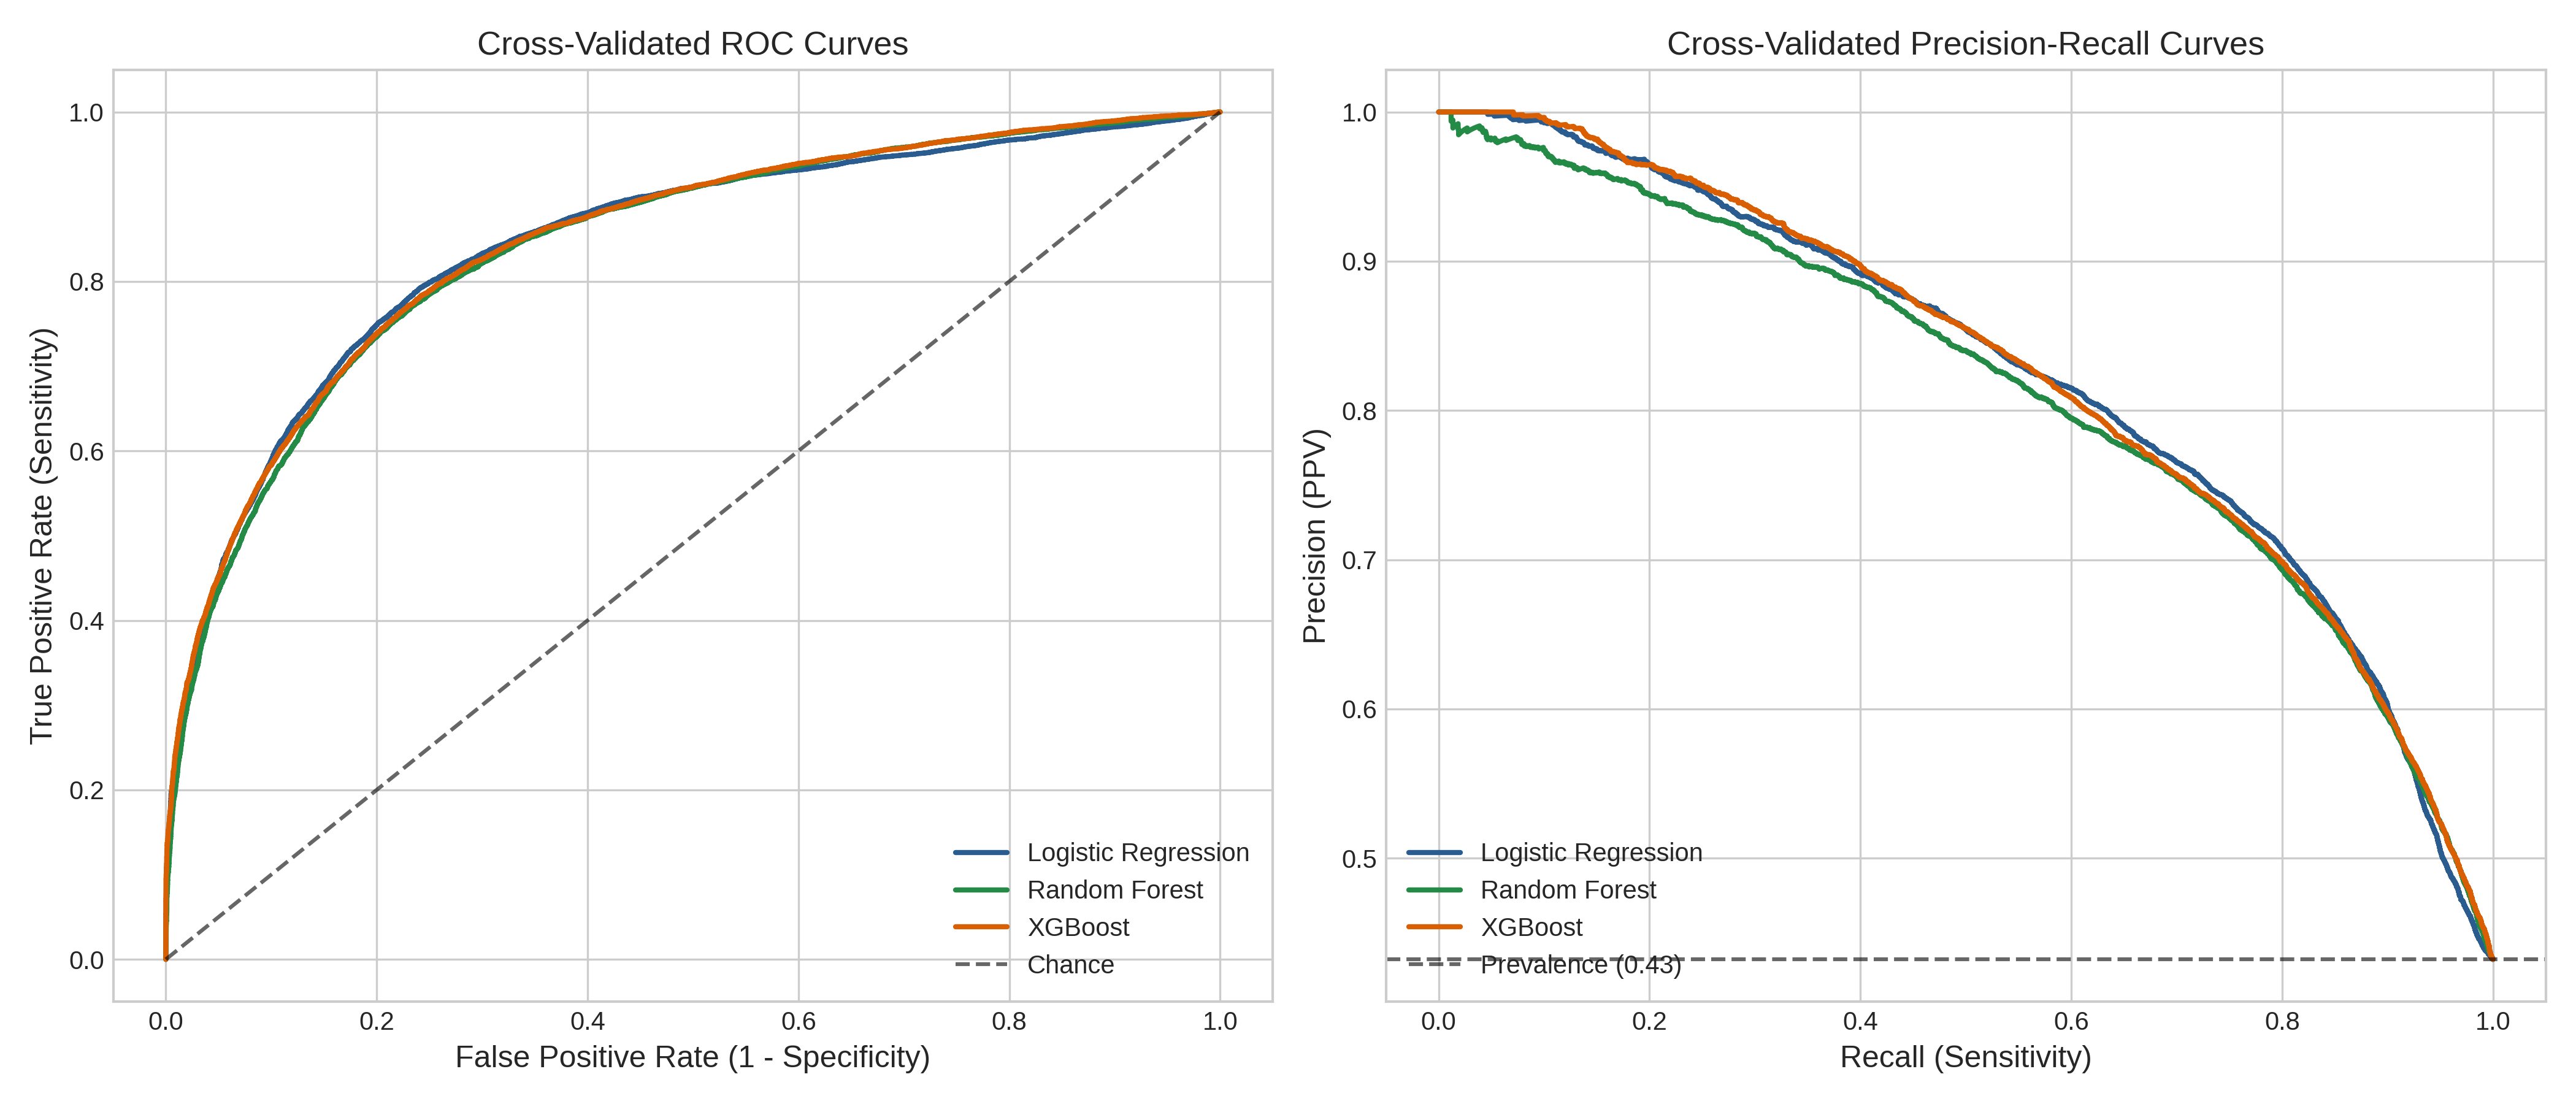
\includegraphics[width=0.88\textwidth]{results/figures/roc_pr_curves.png}
\caption{Receiver Operating Characteristic (ROC) and Precision-Recall (PR) curves across 25 cross-validation folds with $\pm 1$ SD confidence bands.}\label{fig:roc_pr}
\end{figure}

XGBoost achieved the highest overall ROC-AUC ($0.8456 \pm 0.0129$) and PR-AUC ($0.8246 \pm 0.0149$), closely matched by L2-regularized Logistic Regression ($0.8441 \pm 0.0123$ and $0.8242 \pm 0.0143$, respectively). Logistic Regression exhibited marginally higher sensitivity ($0.7303$ vs $0.7025$) and F1-score ($0.7398$ vs $0.7280$). Probabilistic predictions were well-calibrated across architectures, with Brier scores around $0.156$.

\subsection{Global SHAP Risk Factor Rankings}
Aggregating SHAP values across all 25 folds yielded consistent biological rankings across model families (Fig.~\ref{fig:shap_imp}). Age was the primary contributor in all models (mean $|\text{SHAP}| \sim 0.14$--$0.17$), followed by blood urea nitrogen, systolic blood pressure, serum uric acid, and diagnosed diabetes. These five variables accounted for over 72\% of total attribution mass across architectures.

\begin{figure}[t]
\centering
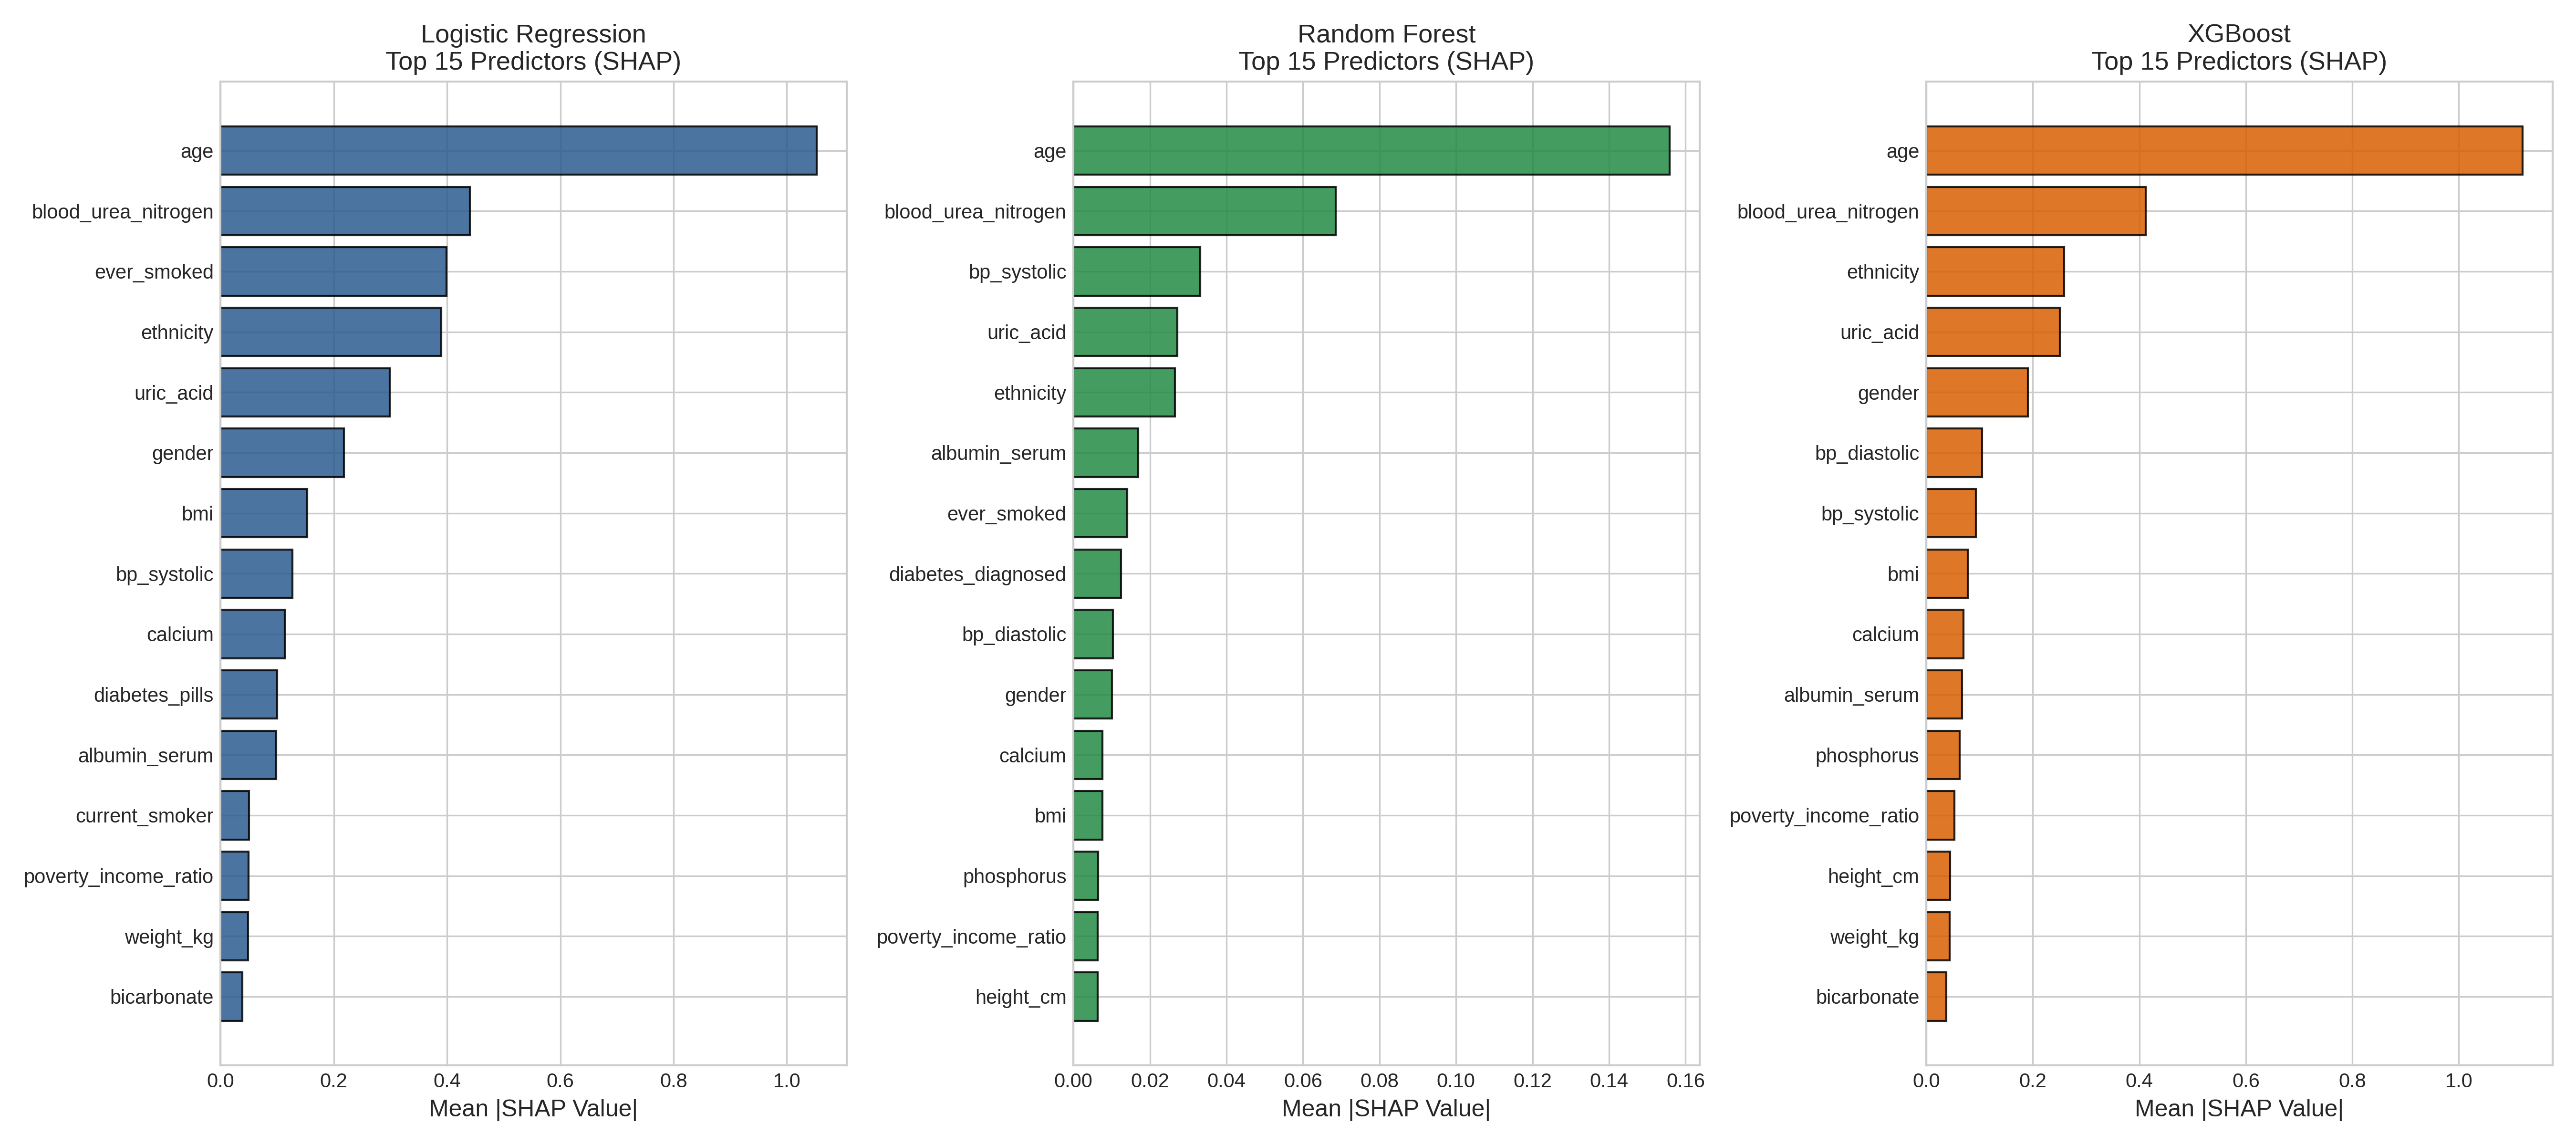
\includegraphics[width=0.88\textwidth]{results/figures/global_feature_importance.png}
\caption{Global SHAP feature importance rankings for Logistic Regression, Random Forest, and XGBoost after dummy-to-parent clinical feature aggregation.}\label{fig:shap_imp}
\end{figure}

\subsection{Explanation Stability Across 300 Fold Pairs}
Evaluating stability across all 300 pairwise fold comparisons showed that tree-based ensembles produced remarkably consistent rankings (Table~\ref{tab:stability}).

\begin{table}[t]
\caption{SHAP attribution stability summary across 300 cross-validation fold pairs.}\label{tab:stability}
\centering
\small
\begin{tabular}{lcccc}
\toprule
Model Architecture & Comparisons & Spearman $\rho$ & Top-5 Jaccard & Top-10 Jaccard \\
\midrule
Random Forest & 300 & $\mathbf{0.9652 \pm 0.0148}$ & $\mathbf{1.0000 \pm 0.0000}$ & $\mathbf{0.9577 \pm 0.0781}$ \\
XGBoost & 300 & $0.9414 \pm 0.0214$ & $\mathbf{1.0000 \pm 0.0000}$ & $0.7997 \pm 0.1087$ \\
Logistic Regression & 300 & $0.8972 \pm 0.0553$ & $0.9267 \pm 0.1383$ & $0.8162 \pm 0.1022$ \\
\bottomrule
\end{tabular}
\end{table}

Random Forest demonstrated the highest ranking stability ($\rho = 0.9652 \pm 0.0148$) and high Top-10 Jaccard consistency ($0.9577 \pm 0.0781$). Both Random Forest and XGBoost achieved a Top-5 Jaccard index of $1.0000 \pm 0.0000$ across all 300 comparisons, showing that the leading five predictors remained invariant to data splits.

\subsection{Missingness Stress Testing}
Models exhibited graceful performance degradation under synthetic MCAR masking (Table~\ref{tab:missingness}).

\begin{table}[t]
\caption{Algorithmic performance and explanation stability under controlled MCAR missingness.}\label{tab:missingness}
\centering
\small
\begin{tabular}{lccccc}
\toprule
Model Architecture & Masking Level & ROC-AUC & F1-Score & Accuracy & SHAP Rank $\rho$ \\
\midrule
Logistic Regression & 0\% (Baseline) & 0.8482 & 0.7422 & 0.7844 & 1.0000 \\
& 10\% MCAR & $0.8366 \pm 0.0023$ & $0.7203 \pm 0.0057$ & $0.7671 \pm 0.0054$ & $0.9403 \pm 0.0037$ \\
& 20\% MCAR & $0.8207 \pm 0.0045$ & $0.7003 \pm 0.0113$ & $0.7501 \pm 0.0108$ & $0.9314 \pm 0.0077$ \\
\midrule
Random Forest & 0\% (Baseline) & 0.8475 & 0.7342 & 0.7804 & 1.0000 \\
& 10\% MCAR & $0.8370 \pm 0.0021$ & $0.7133 \pm 0.0061$ & $0.7679 \pm 0.0041$ & $\mathbf{0.9748 \pm 0.0052}$ \\
& 20\% MCAR & $0.8227 \pm 0.0028$ & $0.6870 \pm 0.0056$ & $0.7528 \pm 0.0054$ & $\mathbf{0.9727 \pm 0.0049}$ \\
\midrule
XGBoost & 0\% (Baseline) & 0.8514 & 0.7264 & 0.7757 & 1.0000 \\
& 10\% MCAR & $0.8385 \pm 0.0029$ & $0.7052 \pm 0.0059$ & $0.7626 \pm 0.0045$ & $0.9590 \pm 0.0103$ \\
& 20\% MCAR & $0.8212 \pm 0.0039$ & $0.6756 \pm 0.0066$ & $0.7439 \pm 0.0075$ & $0.9501 \pm 0.0111$ \\
\bottomrule
\end{tabular}
\end{table}

At 10\% missingness, ROC-AUC declined by roughly 0.011--0.013 points across models. At 20\% missingness, all architectures retained an ROC-AUC above 0.820. SHAP rankings remained congruent with unmasked baselines, maintaining Spearman correlations above 0.930.

\section{Discussion and Conclusion}
The top variables identified by SHAP align directly with established nephrological mechanisms:
\begin{itemize}
    \item \textbf{Chronological Age}: Progressive nephron involution and vascular stiffness reduce functional renal reserve after the fourth decade of life~\cite{denic2016}.
    \item \textbf{Blood Urea Nitrogen (BUN)}: As an end-product of protein metabolism cleared by glomerular filtration, BUN serves as an informative surrogate marker of clearance capacity in the absence of creatinine.
    \item \textbf{Systolic Blood Pressure}: Elevated systemic pressure exposes glomerular microvessels to mechanical barotrauma, accelerating sclerotic changes~\cite{chobanian2003}.
    \item \textbf{Serum Uric Acid}: Hyperuricemia induces renal vasoconstriction, activates the renin-angiotensin system, and promotes tubular epithelial oxidative injury~\cite{johnson2018}.
    \item \textbf{Diabetes}: Diabetic glomerulosclerosis represents the leading global etiology of chronic kidney failure.
\end{itemize}

Contrary to concerns regarding explanation volatility, TreeSHAP applied to Random Forest and XGBoost showed high ranking stability across resampled partitions ($\rho > 0.94$; Top-5 Jaccard = 1.000). The slight variability observed in Logistic Regression ($\rho \approx 0.897$) stemmed primarily from collinearity between blood pressure and glycemic markers, which can shift regression coefficients under small sample shifts.

Several boundary conditions apply to our findings. First, NHANES provides single-timepoint measurements, which cannot confirm whether renal abnormalities persist for three months as required by strict KDIGO definition~\cite{kdigo2024}. The models therefore perform cross-sectional classification rather than longitudinal onset forecasting. Second, excluding direct filtration markers avoids tautology but imposes an upper bound on discrimination ($\text{ROC-AUC} \approx 0.85$). These models are intended for opportunistic risk screening before renal panels are ordered. Third, our stress test evaluated MCAR mechanisms, whereas routine clinical missingness may follow Missing Not at Random (MNAR) patterns.

In conclusion, machine learning classifiers trained on non-leaking clinical and demographic variables achieved an ROC-AUC of approximately 0.846 for concurrent CKD classification in the NHANES 2021--2023 cohort. TreeSHAP feature rankings demonstrated high stability across cross-validation resamples and exhibited graceful degradation under synthetic missingness. The identified consensus factors reflect established pathophysiological pathways, confirming that leak-free opportunistic screening is feasible and that tree-based Shapley explanations provide dependable feature attributions across data perturbations.

\begin{thebibliography}{10}
\bibitem{kdigo2024}
KDIGO Board: KDIGO 2024 Clinical Practice Guideline for the Evaluation and Management of Chronic Kidney Disease. Kidney Int. \textbf{105}(4S), S117--S314 (2024)

\bibitem{bikbov2020}
Bikbov, B., et al.: Global, regional, and national burden of chronic kidney disease, 1990--2017. Lancet \textbf{395}(10225), 709--733 (2020)

\bibitem{inker2021}
Inker, L.A., et al.: New Creatinine- and Cystatin C--Based Equations to Estimate GFR without Race. N. Engl. J. Med. \textbf{385}(19), 1737--1749 (2021)

\bibitem{kovesdy2022}
Kovesdy, C.P.: Epidemiology of chronic kidney disease: an update 2022. Kidney Int. Suppl. \textbf{12}(1), 7--11 (2022)

\bibitem{he2025}
He, T., et al.: Machine learning for screening and risk stratification of chronic kidney disease. Lancet Digit. Health \textbf{7}(2), e104--e115 (2025)

\bibitem{song2024}
Song, X., et al.: Robust machine learning prediction of chronic kidney disease progression using real-world clinical data. JAMIA \textbf{31}(3), 621--632 (2024)

\bibitem{moons2025probast}
Moons, K.G.M., et al.: PROBAST+AI: Risk of Bias Assessment Tool for Prediction Models using Artificial Intelligence. Nat. Med. \textbf{31}(1), 112--128 (2025)

\bibitem{lundberg2017}
Lundberg, S.M., Lee, S.I.: A Unified Approach to Interpreting Model Predictions. In: NeurIPS, vol. 30, pp. 4765--4774 (2017)

\bibitem{nandy2021}
Nandy, P., et al.: On the Stability of Feature Attributions Across Resampled Training Sets in Medical ML. IEEE TNNLS \textbf{32}(8), 3410--3422 (2021)

\bibitem{han2022}
Han, T., et al.: Which Explanation Should I Choose? A Survey and Empirical Evaluation of Explanation Stability and Faithfulness. In: NeurIPS Datasets and Benchmarks (2022)

\bibitem{collins2024tripod}
Collins, G.S., et al.: TRIPOD+AI Statement: Updated Guidance for Reporting Clinical Prediction Models That Use Artificial Intelligence. BMJ \textbf{385}, e078378 (2024)

\bibitem{cdc2024}
Centers for Disease Control and Prevention: NHANES 2021--2023 Documentation. U.S. Dept. of Health and Human Services (2024)

\bibitem{denic2016}
Denic, A., et al.: Structural and Functional Changes With the Aging Kidney. Adv. Chronic Kidney Dis. \textbf{23}(1), 19--28 (2016)

\bibitem{chobanian2003}
Chobanian, A.V., et al.: Seventh Report of the Joint National Committee on High Blood Pressure. Hypertension \textbf{42}(6), 1206--1252 (2003)

\bibitem{johnson2018}
Johnson, R.J., et al.: Hyperuricemia, Acute and Chronic Kidney Disease, Hypertension, and Cardiovascular Disease. Am. J. Kidney Dis. \textbf{71}(6), 851--865 (2018)
\end{thebibliography}

\end{document}
